% Copyright (C) Royal Astronomical Society 2015
% Authors:
% Keith T. Smith (Royal Astronomical Society)

% Change log
%
% v3.0 May 2015
%    Renamed to match the new package name
%    Version number matches mnras.cls
%    A few minor tweaks to wording
% v1.0 September 2013
%    Beta testing only - never publicly released
%    First version: a simple (ish) template for creating an MNRAS paper

%%%%%%%%%%%%%%%%%%%%%%%%%%%%%%%%%%%%%%%%%%%%%%%%%%
% Basic setup. Most papers should leave these options alone.
\documentclass[usenatbib]{mnras}

% MNRAS is set in Times font. If you don't have this installed (most LaTeX
% installations will be fine) or prefer the old Computer Modern fonts, comment
% out the following line
\usepackage{newtxtext,newtxmath}
\usepackage{float}
% Depending on your LaTeX fonts installation, you might get better results with one of these:
%\usepackage{mathptmx}
%\usepackage{txfonts}

% Use vector fonts, so it zooms properly in on-screen viewing software
% Don't change these lines unless you know what you are doing
\usepackage[T1]{fontenc}
\usepackage{ae,aecompl}
%\usepackage[notref,notcite]{showkeys}
\usepackage{color}

%%%%% AUTHORS - PLACE YOUR OWN PACKAGES HERE %%%%%

% Only include extra packages if you really need them. Common packages are:
\usepackage{graphicx}	% Including figure files
\usepackage{amsmath}	% Advanced maths commands
\usepackage{amssymb}	% Extra maths symbols
\usepackage{newtxtext,newtxmath}
\DeclareMathSymbol{v}{\mathord}{lettersA}{51}
%%%%%%%%%%%%%%%%%%%%%%%%%%%%%%%%%%%%%%%%%%%%%%%%%%

%%%%% AUTHORS - PLACE YOUR OWN COMMANDS HERE %%%%%

% Please keep new commands to a minimum, and use \newcommand not \def to avoid
% overwriting existing commands. Example:
%\newcommand{\pcm}{\,cm$^{-2}$}	% per cm-squared

%%%%%%%%%%%%%%%%%%%%%%%%%%%%%%%%%%%%%%%%%%%%%%%%%%

\graphicspath{./Figures/}

%%%%%%%%%%%%%%%%%%% TITLE PAGE %%%%%%%%%%%%%%%%%%%

% Title of the paper, and the short title which is used in the headers.
% Keep the title short and informative.
\title[\textit{aztekas}-HD]{\textit{aztekas}: a GPL hydrodynamic numerical code}

% The list of authors, and the short list which is used in the headers.
% If you need two or more lines of authors, add an extra line using \newauthor
\author[Aguayo-Ortiz, Mendoza \& Tejeda]{
A. Aguayo-Ortiz,$^{1}$\thanks{E-mail: aaguayo@astro.unam.mx}
S. Mendoza$^{1}$\thanks{sergio@astro.unam.mx} and
E. Tejeda,$^{2}$\thanks{emilio.tejeda@conacyt.mx}
\\
% List of institutions
$^{1}$Instituto de Astronm\'ia, Universidad Nacional Aut\'onoma de M\'exico, AP 70-264, Ciudad de M\'exico 04510, M\'exico \\
$^{2}$Universidad Michoacana\\
}

% These dates will be filled out by the publisher
\date{Accepted XXX. Received YYY; in original form ZZZ}

% Enter the current year, for the copyright statements etc.
%\pubyear{2019}

% Don't change these lines
\begin{document}
\newcommand{\diff}{\mathrm{d}}
%\label{firstpage}
%\pagerange{\pageref{firstpage}--\pageref{lastpage}}
\maketitle

%%%%%%%%%%%%%%%%%%%%%%%%%%%%%%%%%%%%%%%%%%%%%%%%%%%%%%%%%%%%
%%%%%%%%%%%%%%%%%%%%%%%% Abstract %%%%%%%%%%%%%%%%%%%%%%%%%%
%%%%%%%%%%%%%%%%%%%%%%%%%%%%%%%%%%%%%%%%%%%%%%%%%%%%%%%%%%%%


\begin{abstract}
This is a simple template for authors to write new MNRAS papers. The abstract should briefly describe the aims, methods, and main results of the paper. It should be a single paragraph not more than 250 words (200 words for Letters). No references should appear in the abstract.
\end{abstract}

% Select between one and six entries from the list of approved keywords.
% Don't make up new ones.
\begin{keywords}
keyword1 -- keyword2 -- keyword3
\end{keywords}
%%%%%%%%%%%%%%%%%%%%%%%%%%%%%%%%%%%%%%%%%%%%%%%%%%%%%%%%%%%%%
%%%%%%%%%%%%%%%%%%%%%%%% Introduction %%%%%%%%%%%%%%%%%%%%%%%
%%%%%%%%%%%%%%%%%%%%%%%%%%%%%%%%%%%%%%%%%%%%%%%%%%%%%%%%%%%%%

\section{Introduction}
\label{sec:intro}


The study of fluid dynamics represents an important
part for the understanding of our universe. Although gravity is the
dominant force in the universe, it is the gas and the plasma, and their
interaction with the gravitational and magnetic fields, the responsible
of a very wide range of astrophysical phenomena. The plasma in the
universe  is the most abundant state of matter.   It can 
be found from stellar up to cosmological scales and the gas dynamics
allows a comprehensive study for  its evolution and behavior.  The
understanding of the coupling with magnetic
fields and radiative processes due to the micro physics of its particles is
essential to model different astronomical observations.

The equations that describe the dynamics of flows are described by the
Euler equations. They constitute a set of non-linear system of hyperbolic
partial differential equations that in most cases have no exact solutions.
This is something very common in physical problems dealing with a set
of partial differential equations.  Usually exact analytic solutions
can be found in cases of highly idealized, symmetrical or self-similar
problems~\citep[see for example][]{landau1987,sedov1959,toro2009,edgar2004} %(\textcolor{red}{CITA
%A LANDAU, ZELDOVICH, TORO, SEDOV, EDGAR}).  
However, in the general
case where more complex scenarios appear, these equations have to be
solved numerically.

Numerical hydrodynamics and, in general, the study of hyperbolic
partial differential equations, constitutes a full branch of study
in physics. Some relevant introductory literature in this topic are the
books by \citet{toro2009}, \citet{leveque2002} and \citet{laney1998},
\textcolor{red}{MAS}.  \textcolor{blue}{The appendix of the article by \citet{aguayo2018} is
a simple comprehensive way in which finite volume methods applied to fluid
dynamics in astrophysics is described.} The continuous search for new and better algorithms to
solve these equations has lead to the development of robust and more accurate
computational codes. These have been used to test and further extend
theoretical models that continuously enrich our understanding of the universe.

In the special case of hydrodynamics, one of the first numerical codes
to be extensively used for astrophysical hydrodynamics is the ZEUS
code~\citep{stone1992}, which uses a finite difference scheme for the
discretization of the differential equations.  Even more, ZEUS has a GNU
Public License (GPL) for its distribution which through the years has made it a
first start for many researchers.  Nowadays more accurate and efficient
numerical methods have been developed reducing computational costs.  Some
of the current hydrodynamical codes that are available to the community are
the following:

\begin{itemize}
  \item PLUTO, reference, description and license.
  \item FLASH, the license use is very restrictive
\end{itemize}

  At the very end it is not only important to have a very robust
hydrodynamical code, but also make it freely available (with a GNU GPL
license or equivalent) to the community, ideally expecting more programmers
to join forces to further improve it.

  In this article we are not aiming at presenting a new different
state-of-the-art code.  Our intention is 
to present and validate our free software (open source, open access)
\textit{aztekas} which has a GNU GPL license, with the aim 
to invite the community to use it and contribue to its development. We also 
include in this article several standard benchmark tests for code
validation, together with the precise form of the algorithms used for its
construction. 



%%%%%%%%%%%%%%%%%%%%%%%%%%%%%%%%%%%%%%%%%%%%%%%%%%%%%%%%%%%
%%% Section: Hyperbolic equations and numerical methods %%%
%%%%%%%%%%%%%%%%%%%%%%%%%%%%%%%%%%%%%%%%%%%%%%%%%%%%%%%%%%%

\section{Hyperbolic equations and numerical methods}
\label{sec:hyper-equations}

%%%%%%%%%%%%%%%%%%%%%%%%%%%%%%%%%%%%%%%%%%%%%%%%%%%%%%%%%%%

\subsection{Finite Volume Method}
\label{subsec:FVM}

The system of partial differential equations in hydrodynamics (HD) and relativistic hydrodynamics (RHD), conforms a set of hyperbolic equations~\citep[see][]{leveque2002}.  These equations can be written in a fully conservative (with no sources terms) or balanced (with  sources terms) form:

%%%%%%%%%%%%%%
%% Equation %%
%%%%%%%%%%%%%%
\begin{equation}
    \frac{\partial \mathbf{q} (\mathbf{u})}{\partial t} + \frac{\partial \mathbf{f}^i (\mathbf{u})}
    {\partial x^i} = \mathbf{s}(\mathbf{u}),
\label{eq:cons-1}
\end{equation}

\noindent where $\mathbf{q}$ are the conservative variables, $\mathbf{f}^i = ( \mathbf{f}^1 , \mathbf{f}^2 , \mathbf{f}^3 )$ are the fluxes of the conservative variables along the three spatial dimensions and $\mathbf{s}$ are the source terms, related to external force (e.g. gravity, cooling functions, etc) or geometrical effects. The vector $\mathbf{u}$ represents the primitive variables of the problem. Each one of these variables $\mathbf{q}$, $\mathbf{f}^i$, $\mathbf{s}$ and $\mathbf{u}$, is a set of $m$ quantities, where $m$ is the number of equations. Finding the solution to this system of equations means to find $\mathbf{u} (t,\bar{x})$. In order to numerically integrate equations~\eqref{eq:cons-1}, the FVM discretization is obtained in the following way. 

Let us begin by considering a three-dimensional domain described in Cartesian coordinates\footnote{The specific case in cylindrical and spherical coordinates is discuss in Appendix~\ref{A:cylsph}}. This domain is then divided into a grid of $N_{x} \times N_{y} \times N_{z}$ cells (or control volumes), centered at $\bar{x}_{i,j,k} = (x_i,y_j,z_j)$, where the subindex $0 \leq i \leq N_x$, $0 \leq j \leq N_y$ and $0 \leq k \leq N_z$, represents the $i$-th, $j$-th and $k$-th position on the grid along each direction. Every cell has a volume $\Delta V := \Delta x \times \Delta y \times \Delta z$, this means that the cell interfaces along, for example, the $x$ direction, are defined at $x_{i + 1/2} := x_i + \Delta x / 2$ and $x_{i - 1/2} := x_i - \Delta x / 2$.

By integrating equation~\eqref{eq:cons-1} over a control volume, we can obtain the semi-discrete form of equation~\eqref{eq:cons-1} for the FVM~\citep[cf.][]{leveque2002,toro2009}:
%%%%%%%%%%%%%%
%% Equation %%
%%%%%%%%%%%%%%
\begin{equation}
\begin{split}
    \frac{\mathrm{d} \mathbf{Q}_{i,j,k}}{\mathrm{d}t} = &- \frac{1}{\Delta x} \left[
    \mathbf{{F}}^x_{i+1/2,j,k} - \mathbf{\hat{F}}^x_{i-1/2,j,k}
    \right]\\
    &- \frac{1}{\Delta y} \left[
    \mathbf{{F}}^y_{i,j+1/2,k} - \mathbf{\hat{F}}^y_{i,j-1/2,k}
    \right]\\ 
    &- \frac{1}{\Delta z} \left[
    \mathbf{{F}}^z_{i,j,k+1/2} - \mathbf{\hat{F}}^z_{i,j,k-1/2}
    \right]\\
    & + \mathbf{S}_{i,j,k},
\end{split}
\label{eq:disc}
\end{equation}

\noindent where we have defined the cell average of $\mathbf{q}$ and $\mathbf{s}$ as
\begin{equation}
    \mathbf{Q}_{i,j,k} := \frac{1}{\Delta V} \int_{x_{i - 1/2}}^{x_{i + 1/2}} \int_{y_{j - 1/2}}^{y_{j + 1/2}}
    \int_{z_{k - 1/2}}^{z_{k + 1/2}} \mathbf{q} (t,\bar{x}) \, \mathrm{d}V,
\end{equation}
\begin{equation}
    \mathbf{S}_{i,j,k} := \frac{1}{\Delta V} \int_{x_{i - 1/2}}^{x_{i + 1/2}} \int_{y_{j - 1/2}}^{y_{j + 1/2}}
    \int_{z_{k - 1/2}}^{z_{k + 1/2}} \mathbf{s} (t,\bar{x}) \, \mathrm{d}V,
\end{equation}

\noindent and the average flux across the cell interface $x_{i + 1/2}$  as
\begin{equation}
    \mathbf{F}_{i+1/2,j,k}^x := \frac{1}{\Delta S_{i+1/2}} \int_{y_{j - 1/2}}^{y_{j + 1/2}} \int_{z_{k - 1/2}}^{z_{k + 1/2}} \mathbf{f}^x(t,\bar{x}_{i+1/2,j,k}) \mathrm{d} S_{i+1/2},
\end{equation}

\noindent where $\Delta S_{i+1/2}$ is the surface normal to $\mathbf{f}^x$ at $x_{i + 1/2 }$. In this particular case $\Delta S_{i+1/2} = \Delta y \Delta z$. For the $x_{i-1/2}$ interface and all the other fluxes, the definition is analogous. 

%Substituting these definitions in the integration of equation~\eqref{eq:cons-1}, we obtain the discretization of the FVM~\citep[cf.][]{leveque2002,toro2009}:

%\noindent where $\Delta t = t_{n+1} - t_n$, $\mathbf{Q}_{i,j,k}^n$ and $\mathbf{S}_{i,j,k}^n$ are the spatial mean value of $\mathbf{q}$ and $\mathbf{s}$, respectively, evaluated at the center of the control volume, at the time $t_n$. On the other hand, $\mathbf{\hat{F}}^i$ are the temporal mean value of the fluxes $\mathbf{f}^i$ along each spatial direction, evaluated at the boundary of the cells. The terms $\Delta x^i$, may vary depending on the specific geometry of the problem. The sub-index $i+1/2,j,k$ means that the flux  is evaluated at $\bar{x}_{i+1/2,j,k} = (x_i^1 + \Delta x^1/2, j , k)$.

The average quantities $\mathbf{Q}_{i,j,k}$ and $\mathbf{S}_{i,j,k}$ may be computed in a simple way as the value of $\mathbf{q}$ and $\mathbf{s}$ at the center of the cell~\citep{leveque2002}. The numerical fluxes $\mathbf{{F}}^i$, on the other hand, are defined at the boundaries of each control volume, so their evaluation must depend on the values of $\mathbf{Q}$ on each side of the interface in which they are defined.

%%%%%%%%%%%%%%%%%%%%%%%%%%%%%%%%%%%%%%%%%%%%%%%%%%%%%%

\subsection{High Resolution Shock Capturing Methods}
\label{susec:HRSC}

%% %% %% %%

\subsubsection{Approximate Riemann Solver}
\label{subsubsec:riemann_solver}

In order to compute the fluxes across the cell interfaces, it is common to use a Godunov-type~\citep{godunov1959} method, which approaches the fluxes by using the information of the conservative variables in a cell and its neighbours. This method consists in solving a Riemann problem at each cell interface.

The Riemann problem consists in an initial data of two constant states divided by an interface. For most hyperbolic systems, this problem can be solved exactly by analyzing the evolution of the solution along the characteristics of the equation~\citep[see][]{toro2009}. If we consider a Riemann problem on the boundary between to contiguous cells at a time $t_m$, it is possible to solve the problem in an exact or approximate form and, from this, obtain an expression for the numerical fluxes. These kind of algorithms are called \textit{Riemann solvers}, and are one of the most commonly used techniques for the so called \textit{high resolution shock capturing} (HRSC) methods.

One the approximate Riemann solver we implemented in \textit{aztekas}, is the HLLE  formula~\citep{hll1983,einfeldt1988}:

%%%%%%%%%%%%%%
%% Equation %%
%%%%%%%%%%%%%%
\begin{equation}  
   \mathbf{{F}} = \left\lbrace
   \begin{array}{ccc}
   \mathbf{f}^L & \mathrm{if} & \lambda_{-} \geq 0, \\
   \frac{\lambda_{+} \mathbf{f}^L - \lambda_{-} \mathbf{f}^R +
   \lambda_{-} \lambda_{+} \left( \mathbf{q}^R - \mathbf{q}^L
\right)}{\lambda_{+} - \lambda_{-}} & \mathrm{if} & \lambda_{-} < 0 <
\lambda_{+} ,\\ 
   \mathbf{f}^R & \mathrm{if} & \lambda_{+} \leq 0 .
   \end{array} 
   \right.
\label{eq:hll}
\end{equation}

\noindent where $\mathbf{f}^{\left\lbrace L,R \right\rbrace}$ and $\mathbf{q}^{\left\lbrace L,R \right\rbrace}$ are the fluxes and conservative variables of the left and right states in the Riemann problem set at the interface between two contiguous cells. This means that, for each control volume, there are two Riemann problems along each direction, one at each boundary $x_{i\pm 1/2}$, $y_{j \pm 1/2}$ and $z_{k \pm 1/2}$. The exact form for computing the right and left state is discuss in Appendix~\ref{A:reconst}.

The values $\lambda_{-}$ and $\lambda_{+}$ represents the characteristic with the larger velocity going to the left and to the right, respectively. These quantities are determined by obtaining the eigenvalues of the Jacobian matrix $\mathcal{B} = \partial \mathbf{f}/ \partial \mathbf{q}$. This scheme turns out to be second order accurate over smooth solutions, but first-order near discontinuities like shock waves~\citep{toro2009}.

The advantage of the HLLE scheme is that, in order to obtain the fluxes, only the eigenvalues of the matrix $\mathcal{B}^i$ are needed, unlike other methods like the Marquina~\citep{marquina1994} or the Roe~\citep{roe1981} approximate Riemman solvers, for which the eigenvectors are also needed. The disadvantage of the HLLE method is its dissipative nature, reason why it does not properly resolves contact discontinuities. To solve this problem, another characteristic velocity based method named HLLC has been developed for both HD~\citep[see][]{toro1994} and RHD~\citep[see][]{mignone2005}. HLLC is less dissipative than HLLE and better resolves the contact discontinuity. Both algorithms for the HD case are included in \textit{aztekas}, and their numerical implementation is discuss in Appendix~\ref{A:hll}.

%%%%%%%%%%%%%%%%%%%%%%%%%%%%%%%%%%%%%%%%%%%%%%%%%%%%%%%%%%%%%%%%%%%%%

\subsubsection{Polynomial Spatial Reconstruction Schemes}
\label{subsubsec:reconst}

As~\citet{delzanna2002} pointed out, when discontinuous solutions are
of main interest, second-order total variation diminishing (TVD) schemes, coupled
with Riemann solvers, are probably the best choice, for obtaining sharp resolution
of discontinuities. In order to do this, we implement in \textit{aztekas}
different types of spatial reconstructions schemes for the primitive variables. We use the
MINMOD~\citep{roe1986}, MC~\citep{vanleer1977} and SUPERBEE~\citep{roe1986}
linear reconstructions, which are second-order methods. We also implement a
fifth-order weighted Essentially Non Oscillatory (WENO5) scheme~\citep{weno2004}, which uses a different approach for the reconstruction that leads to a better capture of discontinuities and non-linear effects~\citep{lora2015}. 

It is not necessary to compute the spatial reconstruction of $\mathbf{u}$ over all the cell. The only values required in order to calculate the fluxes via a Riemann solver are the values ones that relay on the interfaces between contiguous control volumes. For each boundary, there have to be estimated the \textit{left} and $\textit{right}$ that generate the states of the Riemann problem.

For example, in order to compute the approximate Riemann solver along the $x^1$ direction, and in complete analogy for $x^2$ and $x^3$, for a cell centered in $\bar{x}_{i,j,k}$, we have to reconstruct the values at $\bar{x}_{i+1/2,j,k}$ and $\bar{x}_{i-1/2,j,k}$. The implementation of  the spatial reconstruction and the algorithms of each scheme are discuss in Appendix~\ref{A:reconst}.

%%%%%%%%%%%%%%%%%%%%%%%%%%%%%%%%%%%%%%%%%%%%%%%%%%%%%%%%%%%%%%

\subsubsection{Time integration}
\label{subsubsec:tstep}

For the temporal integration, we can write the FVM semi-discrete form as:

%%%%%%%%%%%%%%
%% Equation %%
%%%%%%%%%%%%%%
\begin{equation}
    \begin{split}
    \frac{\diff \mathbf{Q}_{i,j,k}}{\diff t} = \mathcal{R}(\mathbf{Q}),
\end{split}
\label{eq:semi-disc}
\end{equation}

\noindent where $\mathcal{R}(\mathbf{Q})$ is the right hand side of equation~\eqref{eq:disc}. In this way, diving the time interval into sub-intervals $[t_n,t_{n+1}]$, we can use an explicit time variation diminishing Runge-Kutta method~\citep{shu1988}, to integrate over time. In \textit{aztekas}, there are implemented the second order:

%%%%%%%%%%%%%%
%% Equation %%
%%%%%%%%%%%%%%
\begin{equation}
\begin{split}
    \mathbf{Q}_{i,j,k}^* &= \mathbf{Q}_{i,j,k}^n + \Delta t \mathcal{R}(\mathbf{Q}^n), \\
    \mathbf{Q}_{i,j,k}^{n+1} &= \frac{1}{2} \left( \mathbf{Q}_{i,j,k}^n + \mathbf{Q}_{i,j,k}^* + \Delta t \mathcal{R}(\mathbf{Q}^*) \right),
\end{split}
\label{eq:rk2}
\end{equation}

%%%%%%%%%%%%%%
%% Equation %%
%%%%%%%%%%%%%%
\noindent and the third order schemes:
\begin{equation}
\begin{split}
    \mathbf{Q}_{i,j,k}^* &= \mathbf{Q}_{i,j,k}^n + \Delta t \mathcal{R}(\mathbf{Q}^n), \\
    \mathbf{Q}_{i,j,k}^{**} &= \frac{1}{4} \left( 3\mathbf{Q}_{i,j,k}^n + \mathbf{Q}_{i,j,k}^* + \Delta t \mathcal{R}(\mathbf{Q}^*) \right), \\
    \mathbf{Q}_{i,j,k}^{n+1} &= \frac{1}{3} \left( 3\mathbf{Q}_{i,j,k}^n + 2\mathbf{Q}_{i,j,k}^{**} + 2\Delta t \mathcal{R}(\mathbf{Q}^{**}) \right),
\end{split}
\label{eq:rk3}
\end{equation}

\noindent where $\Delta t$ is the time-step, that is usually computed using the standard CFL criterion~\citep{cfl1928} formula:

%%%%%%%%%%%%%%
%% Equation %%
%%%%%%%%%%%%%%
\begin{equation}
    \Delta t = \mathcal{C} \times \mathrm{min} \left( \frac{\Delta x}{\mathrm{max}(|\lambda^x_\pm|)},\frac{\Delta y}{\mathrm{max}(|\lambda^y_\pm|)},\frac{\Delta z}{\mathrm{max}(|\lambda^z_\pm|)} \right),
    \label{eq:cfl}
\end{equation}

\noindent where $\mathrm{max}(|\lambda_\pm|)$ are the maximum absolute value of the characteristic velocity along each direction and $\mathcal{C}$ is the Courant number~\citep[see][]{cfl1928}, which has a typical value less than 1.

\subsubsection{Primitive Variable Recovery}
\label{subsubsec:primitiverecovery}

After the temporal evolution of the conservative variables, the primitive variables need to be recovered. This  step depends on the functional form of $\mathbf{q}$, and on whether or not it is possible to obtain $\mathbf{u}(\mathbf{q})$ analytically. In the case there is not an analytic recovery of the primitive variables, like in the RHD case, a transcendental algebraic equation has to be solved~\citep{riccardi2008}. 

A different approach to overcome this, sometimes, thorny step, is the Primitive Variable Recovery Scheme (PVRS)~\citep[see][]{aguayo2018}, in which a direct time integration over the primitive variables is performed. The semi-discrete form of the PVRS is written as~\citep{aguayo2018}:
%mantaining the same traditional flux reconstruction, like the one presented above but, instead of recovering the primitive variables from the conservative ones solving an algebraic system of equations, the method consist on left-multiplying $\mathcal{L}(\mathbf{Q})$ by the matrix $\mathcal{A} = (\partial \mathbf{q}/\partial \mathbf{u})^{-1}$. The formal discretization of the PVRS is written as~\citep{aguayo2018}:

%%%%%%%%%%%%%%
%% Equation %%
%%%%%%%%%%%%%%
\begin{equation}
\begin{split}
    \frac{\mathrm{d} \mathbf{U}_{i,j,k}}{\mathrm{d}t} =  &- \frac{1}{\Delta x} \mathcal{A}_{i,j,k} \cdot \left[
    \mathbf{F}^x_{i+1/2,j,k} - \mathbf{\hat{F}}^x_{i-1/2,j,k}
    \right]\\
    &- \frac{1}{\Delta y} \mathcal{A}_{i,j,k}^n \cdot \left[
    \mathbf{F}^y_{i,j+1/2,k} - \mathbf{{F}}^z_{i,j-1/2,k}
    \right]\\ 
    &- \frac{1}{\Delta x^3} \mathcal{A}_{i,j,k}^n \cdot \left[
    \mathbf{F}^z_{i,j,k+1/2} - \mathbf{F}^z_{i,j,k-1/2}
    \right]\\
    & + \mathcal{A}_{i,j,k} \cdot \mathbf{S}_{i,j,k} := \mathcal{R}(\mathbf{U}),
\end{split}
\label{eq:pvrs}
\end{equation}

\noindent where $\mathbf{U}_{i,j,k}$ is the cell average value of the primitive variables $\mathbf{u}$, $\mathcal{A}_{i,j,k} := (\partial \mathbf{q}/\partial \mathbf{u})^{-1}$ and where the numerical fluxes $\mathbf{F}$ may be computed using an approximate Riemann solver. This algorithm is also implemented in \textit{aztekas} and is used for some numerical tests presented in this work.

\subsubsection{Ghost cells}
\label{subsubsec:ghost}

In order to implement the boundary conditions, it is necessary to extend the numerical domain further away from the original region of interest. These extended cells are often referred as \textit{ghost cells}~\citep[see for example][]{leveque2002,hindenlang2019}. The number of ghost cells needed for a problem depends on the stencil used to reconstruct the primitive variables. For example, for linear reconstructions as MINMOD or MC, only 1 ghost cells is needed for the boundary conditions, but for a WENO5 reconstruction, which uses three stencils of three cells each, at least three ghost cells are needed in order implement the boundary conditions.
%%%%%%%%%%%%%%%%%%%%%%%%%%%%%%%%%%%%%%%%%%%%%%%%%%%%%%%%%%%%%%%
%%%%%%%%%%%%%%%%%%%%%%%%%% Hydrodynamics %%%%%%%%%%%%%%%%%%%%%%
%%%%%%%%%%%%%%%%%%%%%%%%%%%%%%%%%%%%%%%%%%%%%%%%%%%%%%%%%%%%%%%
\section{Hydrodynamics}
\label{sec:HD}

The Euler equations in the non-relativistic regime written in a balanced
form are~\citep[see][]{landau1987} (using Einstein notation):

%%%%%%%%%%%%%%%
%% Equations %%
%%%%%%%%%%%%%%%
\begin{equation}
    \frac{\partial \rho}{\partial t} + \nabla_j \left( \rho u^j \right) = 0,
\end{equation}
\begin{equation}
    \frac{\partial E}{\partial t} + \nabla_j \left[ (E + p) u^j \right] = \Gamma
    - \Lambda + f_j u^j,
\end{equation} 
\begin{equation}
    \frac{\partial \left( \rho u^i \right)}{\partial t} + \nabla_j \left( \rho
    u^i u^j \right) + \nabla^i p = f^i,
\end{equation} 

\noindent where $\rho$ is the mass density, $u^i = \mathrm{d}x^i/\mathrm{d}t$ is
the velocity vector, $p$ is the pressure and $E$ is the total energy density.
We define the covariant derivative $\nabla_i$
inverse three-dimensional metric tensor is defined as
$\gamma^{ij}$, and so $\nabla^j = \gamma^{ij} \nabla_i$, $\Gamma -
\Lambda$ represents the net energy gain/loss per unit volume and $\vec{f}$
are the external forces per unit of mass acting on the fluid, such as gravity.

In order to close the system, we need an equation for the total energy
density. In general,

%%%%%%%%%%%%%%
%% Equation %%
%%%%%%%%%%%%%%
\begin{equation}
    E = \frac{1}{2}\rho\, (u_j u^j) + \rho \epsilon,
\end{equation}

\noindent where we define $u_i = \gamma_{ij}u^j$ and $\epsilon$ is the internal energy of
the fluid, which follows an equation of state (EoS) of the form $\epsilon =
\epsilon(\rho,p)$. For \textit{aztekas}, we adopted a polytropic EoS:
%%%%%%%%%%%%%%
%% Equation %%
%%%%%%%%%%%%%%
\begin{equation}
    \epsilon = \frac{p}{\rho (\gamma - 1)},
\end{equation}

\noindent where $\gamma$ is the polytropic index of the gas. Different and
more realistic both analytic and numerical EOS had been developed to study
either gases~\citep[cf.][]{ryu2006} or more complex systems like neutron
stars~\citep[cf.][]{zhu2018}, but the polytropic gas approximation remains
a valid and good approximation for many astrophysical phenomena.

The primitive and conservative variables, as well as the fluxes and sources
terms for this system, using index  $i$ to represent one specific flux
direction and $j$ all three spatial directions, are:

%%%%%%%%%%%%%%%
%% Equations %%
%%%%%%%%%%%%%%%
\begin{equation}
    \mathbf{u} = \left( \rho, p, v^j \right),
\end{equation}
\begin{equation}
    \mathbf{q} = \left( \rho, E, \rho v^j \right),
\end{equation}
\begin{equation}
    \mathbf{f}^i = \left( \rho v^i, [E + p]v^i, \rho v^i v^j + p\delta^{ij} \right),
\end{equation}

\noindent and

\begin{equation}
    \mathbf{s} = \left( 0, \Gamma - \Lambda + \vec{f}\cdot \vec{v}, f^j \right).
\end{equation}

\noindent where $v^j$ is the physical velocity vector, which is related with $u^j$ as
\begin{equation}
    v^j = \sqrt{\gamma_{(jj)}} u^j,
\end{equation}

\noindent where $\gamma_{(jj)}$ are the three-dimensional metric components along the diagonal (no implicit sumation is intended).

%%%%%%%%%%%%%%%%%%%%%%%%%%%%%%%%%%%%%%%%%%%%%%%%%%%%
%%%%%%%%%%%%%%%%% Code Validation %%%%%%%%%%%%%%%%%%
%%%%%%%%%%%%%%%%%%%%%%%%%%%%%%%%%%%%%%%%%%%%%%%%%%%%


\section{\textit{aztekas} code validation}
\label{sec:codevalid}

In order to validate \textit{aztekas} for its research usage, in this section we present a number of numerical tests and comparison with analytic solutions in the non-relativistic regime. All simulations presented here were computed using a second order Runge-Kutta method. The specific flux calculation, Courant number, primitive variable reconstruction and recovery, will be specified at each test.

\begin{table}
    \centering
    \caption{Initial parameters for the four tests of the 1D shock tube problem. The labels $L$ and $R$ represent the initial left and right states, respectively.}
    \begin{tabular}{c|cccc}
    \hline 
    Parameters & Test 1 & Test 2 & Test 3 & Test 4  \\
    \hline 
    $\rho_L$ & 1.0   & 10.0  & 1.0  & 5.0 \\
    $p_L$    & 1.0   & 13.33 & 0.2  & 1.0 \\
    $v_L$    & 0.0   & 0.0   & -1.5 & 0.5 \\
    $\rho_R$ & 0.125 & 1.0   & 1.0  & 1.0 \\
    $p_R$    & 0.1   & 0.01  & 0.2  & 1.0 \\
    $v_R$    & 0.0   & 0.0   & 1.5  & 0.0 \\
    $\gamma$ & 5/3   & 5/3   & 5/3  & 1.4 \\
    \hline
    \end{tabular}
    \label{tab:sod}
\end{table}

%%%%%%%%%%%%%%% Shock Tube %%%%%%%%%%%%%%%%%

\subsection{Shock tube}
\label{subsec:sod}

\subsubsection{One dimensional shock tube}
\label{subsubsec:shock}

The shock tube test, first presented by~\citet{sod1978}, consists on a Riemann problem along the entire integration domain. The 1D problem has an exact solution which is presented, for the non-relativistic case, by~\citet{toro2009}. This test has also been performed with \textit{aztekas} using the PVRS discretization~\eqref{eq:pvrs} in the relativistic regime~\citep[see][]{aguayo2018}.

The numerical solution was computed for various test, changing the initial density, pressure and velocity. All the results presented for the Shock tube test use the HLLE formula, a MC limiter for the linear reconstruction of the primitive variables, a domain [0,1] with $N = 400$ identical cells, and a Courant number of 0.9. The initial discontinuity is placed at $x = 0.5$. Unless it is specified, all simulations where performed using the classical primitive variable recovery, this is, $\mathbf{u}$ is recover directly from $\mathbf{q}$.

\begin{figure}
    \centering
    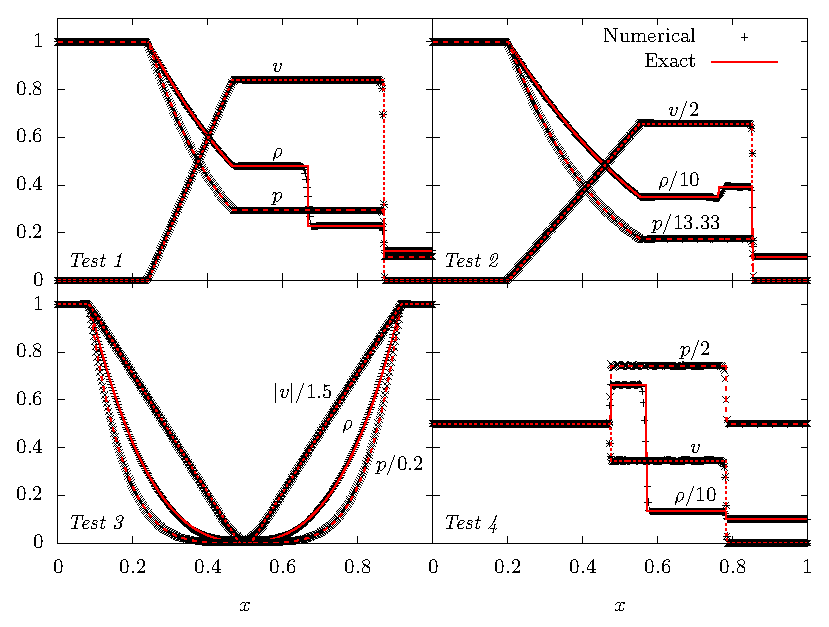
\includegraphics[width=0.47\textwidth]{Figures/sodtests.eps}
    \caption{Results of the 1D shock tube tests for the four sets of initial conditions listed in Table~\ref{tab:sod}. Each panel corresponds to a different test and compares the density, pressure and velocity as obtained against their corresponding analytic values. In all cases t=0.2.}
    \label{fig:sodtests}
\end{figure}

\begin{figure}
    \centering
    \includegraphics[width=0.47\textwidth]{Figures/lnorm.eps}
    \caption{$L^1-$norm of the error in the density versus the resolution $N$ for all tests presented in Table~\ref{tab:sod}. In a dotted line, for comparison, we present the slope that a first order of convergence must have.}
    \label{fig:lnorm}
\end{figure}


In Table~\ref{tab:sod} we show the initial parameters for the left ($x < 0.5$) and right ($x > 0.5$) state of the shock tube problem. These tests were selected in order to obtain different kind of intermediate states. In Test 1 and 2 two different type of working surface with a rarefaction wave are created, in Test 3 two rarefaction waves induces a lower density zone and in Test 4 a strong shock without a rarefaction wave is formed. The boundary conditions wer set as free outflow in both directions by copying the value of the last evolved cell onto the adjacent ghost cells (zero order extrapolation).

%with a rarefaction wave were created (Test 1 and 2), two rarefaction waves induces a lower density zone (Test 3) and were a strong shock without rarefaction wave is formed (Test 4). The boundary conditions were set as outflow in both directions, and this was computed by doing a zero order extrapolation to the ghost cells, i.e., by setting the value of the last valid control volume to all ghost cells.ex

In Figure~\ref{fig:sodtests} we show the density, pressure and velocity at a time $t=0.2$ for the four tests. The figure shows the results of the numerical simulations compared against the corresponding exact, analytic values~ \citep{toro2009}. As can be seen from this figure, for all cases there is a good agreement between the numerical and the analytic solutions all over the domain.

In order to determine the convergence rate of the code, we repeated the same four tests presented in Table~\ref{tab:sod}, using six different resolutions $N_1 = 100$, $N_2 = 200$, $N_3 = 400$, $N_4 = 800$, $N_5 = 1600$ and $N_6 = 3200$. We compute the $L_1$ norm of the error between the numerical and the analytical solution. The order of convergence $Q$ is estimated as 
\begin{equation}
Q \approx \frac{\log(e_{i+1}/e_i)}{\log(\Delta x_{i+1}/\Delta x_i)},
\end{equation}

\noindent where $e_i$ is the $i$-th error obtained for the $\Delta x_i$ resolution. The result is shown in Figure~\ref{fig:lnorm} and, as expected due to the presence of discontinuities (see Section~\ref{subsubsec:riemann_solver}), the order of convergence is $\sim 1$ for all tests, due to the presence of discontinuities.

%%%%%%%%% Shock tube - Cyl and Sph %%%%%%%%%%

\subsubsection{Shock tube test in cylindrical and spherical coordinates}
\label{subsubsec:sodcylsph}

\begin{figure}
    \centering
    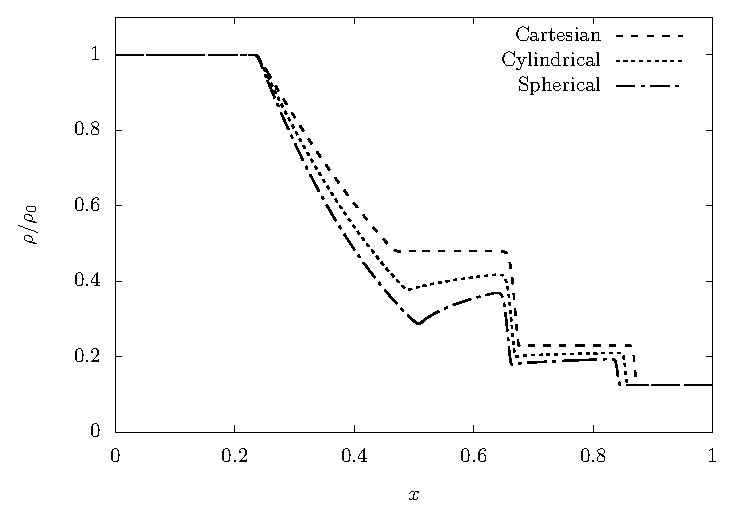
\includegraphics[width=0.47\textwidth]{Figures/comb.eps}
    \caption{Comparison of the density profile in Cartesian, cylindrical and spherical coordinates for the Test 1 in Table~\ref{tab:sod}.}
    \label{fig:comp}
\end{figure}

In addition to Cartesian coordinates, we have also implemented within \textit{aztekas} the use of cylindrical and spherical coordinate systems. In this Subsection, we present the results of the 1D shock tube test for these geometries. This kind of tests have been done presented by other authors~\citep[e.g.][]{radice2012,lora2015}, although it is not commonly considered as part of a test suite because as a numerical suited test because there are not analytic solutions to this problem in spherical and cylindrical geometries. All simulations for this case were done with a HLLE flux calculator, the MC reconstruction, the standard primitive variable recovery and a grid of $N=400$ points.

In Figure~\ref{fig:comp} we show the results of the density in this test for the spherical and cylindrical versions of Test 1 in Table~\ref{tab:sod} at $t=0.2$. For comparison, we also show in this figure the result obtained with Cartesian coordinates discussed in the previous Subsection. As can be seen, due to geometrical source terms in the balanced equations (see Appendix~\ref{A:cylsph}), the form of the density profile differs in all cases. 
%In particular, 1D spherical simulations are really useful for problems with a complete spherical symmetry, as would be seen below with the spherical accretion tests.


%%%%%%% Multidim - Shock Tube %%%%%%%%%

\subsubsection{Two dimensional shock tube}
\label{subsubsec:2dsod}

\begin{figure}
    \centering
    \includegraphics[width=0.47\textwidth]{Figures/shock-d.png}
    \caption{Density profile of an initial configuration of Test 1 with an interface located at $x + y = 1$ at time $t = 0.2$.}
    \label{fig:diag}
\end{figure}
\begin{figure}
    \centering
    \includegraphics[width=0.47\textwidth]{Figures/diag.eps}
    \caption{Density, pressure and velocity profile along the diagonal $x=y$, compared with the exact solution.}
    \label{fig:diag-1d}
\end{figure}

We performed the shock tube problem for one of the tests of Table~\ref{tab:sod} along a diagonal in a $400 \times 400$ cartesian grid in order to analyze the flux calculation along two dimensions simultaneously.~\citep[see][were a similar study was implemented for the relativistic case]{lora2015}.

\begin{figure*}
    \centering
    \includegraphics[width=0.95\textwidth]{Figures/reflection.png}
    \caption{Isocontour density plot of the double mach reflection at a time $t=0.25$.}
    \label{fig:reflection}
\end{figure*}

In Figure~\ref{fig:diag} we show the snapshot of the shock tube evolution at time $t=0.2$ for the Test 1 of Table~\ref{tab:sod}. We use the HLLC flux formula, the MC limiter and the standard primitive variable recovery. The left and right states were delimited by a line with equation $x + y = 1$. The boundary conditions were set as outflow in all directions. For this case we implemented a linear extrapolation to the ghost cells in the boundaries in order to avoid spurious reflections. Although, as can be seen from Figure~\ref{fig:diag}, the solution still shows a problem in the boundaries, specifically at the bottom-right and upper-left corners, where a small diminishing in the density is observed. It is likely that this is because the extrapolation was done independently for each direction. In Figure~\ref{fig:diag-1d} we show the density, pressure and velocity profile along the diagonal $x=y$, and compare the numerical results against the analytic solution.


\subsection{Double Mach reflection}
\label{subsec:strongshock}

The HRSC methods are designed not only for the accurate resolution of the position and sharpness of discontinuities, like shock waves, but also to avoid spurious numerical instabilities, as the \textit{carbuncle instability}~\citep{rodionov2018}\footnote{Some authors~\citep[e.g.]{moschetta2001} claim that, rather to be a numerical pathology, the carbuncle instability is intrinsically associated to the Euler equations.}. This instability appears when a shock wave interacts with other shocks or reflecting walls, and manifests as a growing protuberance ahead of the discontinuity. This spurious problem seems to appear when a less dissipative method is used in the simulation~\citep{woodward1984}.

The double Mach reflection test was first described by~\citet[][]{woodward1984}, and it is part of some codes test suite~\citep[e.g.]{stone2008}. The problem consists on a strong shock wave moving diagonally toward a reflecting wall.
Although there is not analytic solution for this problem, is a commonly used problem for testing that shocks propagate at the correct speed in all directions (avoid the carbuncle instability) and the proper reflective boundaries implementation.

In order to test the stability of the solution, this test was performed using the WENO5 reconstructor and the HLLC flux calculator, which is a less dissipative method (compare with the HLLE). We also performed a high resolution simulation on a Cartesian domain $[0,4]\times[0,1]$, with $1200\times300$ uniformly distributed grid cells. We use a polytropic index $\gamma = 1.4$, the standard primitive variable recovery and a Courant number of 0.5.

Our initial and boundary conditions closely follows those by~\citet{stone2008}. The domain was divided into a pre-shock and post-shock region, delimited by a discontinuity that forms a 60$^\circ$ angle with the $x$-axis, intersecting it at $x_0 = 1/6$. The shock zone moves diagonally towards the lower boundary with a Mach number of 10, so the initial conditions are

 \begin{equation}
     \left( \rho, p \right) = \left\lbrace
     \begin{array}{cl}
        (8,116.5) & \mathrm{if}\, x < x_0 + y/\sqrt{3} \\
        (1.4,1) &   \mathrm{if}\, x \geq x_0 + y/\sqrt{3},
     \end{array}
     \right.
 \end{equation}
 
\noindent with velocity components for the post-shock zone
\begin{equation}
    \begin{split}
        v_x &= 8.5 \cos(30^\circ), \\
        v_y &= -8.5 \sin(30^\circ),
    \end{split}
\end{equation}

\noindent and the pre-shock zone initially at rest.

We set free outflow conditions at the left and right boundaries and reflection at the lower boundary for $x > x_0$. For $x < x_0$ we fill the ghost cells with the values of the post-shock zone. For the upper boundary, we impose the ghost cells to follow the movement of the diagonal shock, so we set the pre-shock conditions for $x \geq x_s(t)$ and the post-shock conditions for $x < x_s(t)$ where
\begin{equation}
    x_s(t) = x_0 + \frac{1 + 20t}{\sqrt{3}},
\end{equation}

\noindent is the position of the shock at the upper boundary. This initial conditions were taken from~\citet{woodward1984}.

In Figure~\ref{fig:reflection} we show the density contour levels of the double mach reflection for a time $t = 0.25$. This result is in good agreement with the one presented in other works~\citep[e.g.][]{she2016}: the contact surface curly jet, that appears along reflecting wall, does not reach the shock front, avoiding the carbuncle instability. 





%%%%%%%%%%%%% Sedov %%%%%%%%%%%%%%%%

\subsection{Sedov blast wave}
\label{subsec:sedov}

The Sedov blast wave~\citep{sedov1959} consists of an intense explosion caused by an enormous amount of energy deposited in a small volume at the center of the domain, which generates a strong spherically symmetric shock which propagates through a homogeneous medium.

This problem was studied by~\citet{sedov1959}, finding a self-similar solution evolves in time as the shock front radius is given by~\citep{sedov1959,landau1987}:
\begin{equation}
    r(t) = \left( \frac{E_0}{\alpha \rho_0} \right)^{1/5} t^{2/5},
    \label{eq:self-sim-sedov}
\end{equation}

\begin{figure}
    \centering
    \includegraphics[width=0.47\textwidth]{Figures/sedov.eps}
    \caption{Comparison between numerical results and the analytic solution of the density, pressure and velocity  for the 2D spherical axisymmetric simulation of the Sedov blast wave. We only plot the profiles along $\theta = \pi/4$ as no angular dependence was shown.}
    \label{fig:sedov}
\end{figure}

\noindent where $E_0$ is the initial energy injected, $\rho_0$ is the background density and $\alpha$ is a constant that depends on the equation of state. This solution is relevant in astrophysics as it helps to understand the physics behind a supernovae explosion. The Sedov blast wave is a commonly used benchmark test for hydrodynamic codes~\citep{tasker2008}.

Continuing with the 2D tests, for this simulation we implement a 2D spherically axisymmetric grid with $400 \times 20$ cells uniformly distributed over a $[0,8]\times[0,\pi/2]$ domain. We use the HLLC flux calculator, the MC reconstructor and a Courant number of 0.25, as well as the standard primitive variable recovery. We set an initial explosion energy of $E_0 = 1.25 \times 10^5$ inside a radius $r_0$ that corresponds to 8 numerical cells near the origin. The initial pressure $p_0$ was computed using the polytropic EoS as
\begin{equation}
    p_0 = \frac{3(\gamma - 1) E_0}{4 \pi \rho_0 r_0^3},
\end{equation}

\noindent were the polytropic index was set to $\gamma = 5/3$. The gas is set initially at rest and $\rho_0 = 1$. The explosion shock front propagates through a static medium with $p_m = 0.00001$ and $\rho_m = \rho_0$. We use free outflow conditions at both inner and outer radial boundaries and reflection along the axis $\theta = 0$ and $\pi/2$.

In Figure~\ref{fig:sedov} we show the density, pressure and velocity profiles of the Sedov explosion at $t=0.1$ along the $\theta = pi/4$ direction. For comparison, we also show the corresponding analytic solution~\citet{kamm2000}. As can be seen, there is a good agreement between the numerical results and the analytic solution, the shock is well resolved, as expected for the HLLC Riemann solver.

In order to determine the convergence rate for this test, we repeated the simulation using different radial resolutions, maintaining the same number of cells along $\theta$. We compute the $L^1-$norm using the standard primitive variable recovery and the PVRS discretization~\eqref{eq:pvrs}. In Figure~\ref{fig:lnorm-sedov}, we show that, for both methods, the order of convergence is $~1$, which is expected due to the strong shock front. For a higher resolution, the convergence rate decreases in both cases, this is the result of the truncation error being dominated by the rounding error\footnote{The truncation error is the difference between the exact solution and a numerical solution obtained with certain method. The rounding error is due to the precision of the computer~\citep[][]{leveque2002}}.

%We repeated this simulation using different radial resolutions, maintaining the same number of cells along $\theta$, in order to calculate the $L^1-\mathrm{norm}$, and in this case we obtain it also using the PVRS discretization~\eqref{eq:pvrs} for the direct primitive variable recovery, as can be seen in Figure~\ref{fig:lnorm-sedov}. As we can see, for both schemes, at low resolution, the convergence is similar, but, as the resolution increases, the convergence is faster for the PVRS. For a higher resolution the convergence order decreases in both cases, this is the result of the truncation error being dominate by the rounding error

\begin{figure}
    \centering
    \includegraphics[width=0.45\textwidth]{Figures/lnorm_sedov.eps}
    \caption{$L^1-$norm of the error between numerical and analytic solution of the Sedov blast wave for resolutions $N_r = 50,\, 100,\, 200,\, 400\, \mathrm{and}\, 800$. We compare here the convergence for different schemes of primitive variable recovery: the standard way, recovering $\mathbf{u}$ directly from $\mathbf{q}$, and the PVRS using discretization~\eqref{eq:pvrs}.}
    \label{fig:lnorm-sedov}
\end{figure}




\subsection{Hydrodynamic instabilities}
\label{subsec:hydinst}

In astrophysics, the non-linear nature of hydrodynamic equations is the responsible of the turbulence presented in different scenarios like stellar atmospheres~\citep[see][]{jeffrey2018} or accretion disks~\citep[see][]{wienkers2018}. It is important for a code to be able to resolve the fine structure of the turbulence in a simulation, since is in this zone were important physical process occur~\citep[eg.][]{duffel2016}. In this subsection we analyze the behavior of \textit{aztekas} in the non-linear regime with two classical tests: the Kelvin-Helmholtz and the Rayleigh-Taylor instabilities~\citep{chandra1981}.

%%%%%%%%%%%%% Kelvin-Helmholtz %%%%%%%%%%%%%%%
\subsubsection{Kelvin-Helmholtz instability}
\label{subsubsec:kh}
\begin{figure*}
    \centering
    \includegraphics[width=0.70\textwidth]{Figures/kelvin-helmholtz.png}
    \caption{Onset of the Kelvin-Helmholtz instability. The panels show the time evolution of the density following a one-mode perturbation on the velocity field (see Eq~\ref{eq:initial-kh}). From top to bottom and left to right, the times are $t = 0.0$, $1.5$, $2.5$ and $3.5$, with an amplitude perturbation $\eta = 0.01$.}
    \label{fig:kelvin-helmholtz}
\end{figure*} 

The Kelvin-Helmholtz (KH) instability is the result of perturbing the interface between two fluids that are moving in opposite directions. This interaction drives the fluid to enter a non-linear regime where the turbulence starts to dominate.
 
The KH instability is a usual phenomenom in astrophysics. It appears at different scales in the Universe, from solar flares~\citep{ruan2018} and molecular clouds~\citep{pandey2019}, up to relativistic jets in active galactic nuclei~\citep{perucho2006} and even at cosmological scales~\citep{malik2003}.
 
This test was performed using the HLLC Riemann solver, the WENO5 primitive variable reconstructor, the standard primitive variable recovery, a Courant factor of $0.5$ and a polytropic index $\gamma = 1.4$. We implemented a cartesian square domain $[-0.5,0.5]\times[-0.5,0.5]$ with an uniform distributed grid of $600\times600$ cells and periodic conditions in all boundaries.
 
We divided the domain into two zones with fluids moving in opposite directions along the $x$ direction. The initial conditions were then set as
 \begin{equation}
     \left( \rho, p, v_x, v_y \right) = \left\lbrace
     \begin{array}{cl}
        (2,2.5,0.5v,\delta v) & \mathrm{if}\, |y| \geq 0.25, \\
        (1,2.5,-0.5v,\delta v) &   \mathrm{if}\, |y| < 0.25,
     \end{array}
     \right.
     \label{eq:initial-kh}
 \end{equation}
 
\noindent where $v = 1 + \delta v$ and $\delta v = \eta \cos(2\pi x/L_x) \sin(2\pi y/L_y)$ is the perturbation, with $\eta$ its amplitude that, in this case, was set to $0.01$. $L_x=1$ and $L_y=1$ are the extension of the domain along each direction. This corresponds to one-mode perturbation for the velocity over the $x-y$ plane.
 
In Figure~\ref{fig:kelvin-helmholtz} we show the resulting time evolution in the density field at times $t = 0.5$, 1, 1.5 and 2. As can be seen from the bottom right panel of the figure, the upper eddies are exactly the same as the ones below, only inverted left to right, i.e. even though a full non-linear regime has been developed, the simulation keeps this symmetry at all times. The fact that there is a clear distinction between the fluids of high and low density shows the non-dissipative nature of the HLLC Riemann solver.

%%%%%%% Rayleight-Taylor %%%%%%%%%%%%%%%
\subsubsection{Rayleigh-Taylor instability}
\label{subsubsec:rt}


 
The Rayleigh-Taylor (RT) instability is the result of perturbing the interface between a high density fluid on the top of a low density fluid with a gravitational force pointing downward. This instability appears in astrophysical scenarios like supernovas where the dense shell, obtained by the explosion, is decelerated by the external medium and the gravity of the remnant star~\citep{fraschetti2010}. The turbulence generated has been shown to be an important mechanism from which the magnetic field is intensified and where the synchrotron radiation is obtained~\citep{duffel2016}.

For this test we use an HLLC Riemann solver, a WENO5 primitive variable recovery, a standard primitive variable reconstruction, although we also use the PVRS scheme to compare; a Courant factor of 0.5 and a polytropic index $\gamma = 1.4$. We set a uniform $300\times900$ spaced grid in a rectangular domain $[-0.25,0.25]\times[-0.75,0.75]$, using periodic conditions in both $x$ boundaries, and reflection in the $y$ boundaries. We also implemented a uniform gravitational acceleration going downward $g = -1$ as a source term.

The domain was divided into two zones with different density fluids. The general initial conditions were set as
 \begin{equation}
     \left( \rho, p, v_x, v_y \right) = \left\lbrace
     \begin{array}{cl}
        (2.0,p_h,0.0,\delta v) & \mathrm{if}\, |y| \geq 0, \\
        (1.0,p_h,0.0,\delta v) &   \mathrm{if}\, |y| < 0,
     \end{array}
     \right.
 \end{equation}
 
 \begin{figure}
     \centering
     \includegraphics[width=0.47\textwidth]{Figures/rt-comp.png}
     \caption{Rayleigh-Taylor instability of a one mode perturbation (left) with an amplitude $\eta=0.01$, and a random perturbation of the same amplitude.}
     \label{fig:rt-1}
 \end{figure}
 
 \noindent where $p_h = 2.5 - \rho g y$, with $g=1$ is the pressure a fluid in hydrostatic equilibrium, in order to balance the forces between pressure gradients and gravity. For the velocity fluctuation $\delta v$, we use a one mode perturbation of the form $- \eta(1 + \cos(2\pi x/L_x)*(1 + \cos(2 \pi y/ L_y )))/4 $, similar to the one use for the KH instability, and a random perturbation.



 In Figure~\ref{fig:rt-1} we show the mass density evolution of the RT instability at a time $t = 3.0$ for the one mode perturbation, with an amplitude $\eta = 0.01$ (left) and a random perturbation of the same amplitude (right). As can be seen in the left image, the fluctuation of the fluid in the interface, along with the constant gravitational field, leads the higher density fluid to stream down without mixing with the lower density one, even though, the KH instability shows up in the layer between both fluids. On the right image, the random perturbation leads the fluid to a mixture that propagates more slowly. In both cases, the transition to non-linear turbulence is observed.

 In Figure~\ref{fig:rt-2} we show the comparison between a one mode perturbation model, with an amplitude $\eta = 0.1$, for the standard finite volume method (left) with the PVRS discretization (right), at a time $t=0.3$. Due to the bigger amplitude of the fluctuation, the higher density fluid sink deeper in the same amount of time. In both cases the non-linear turbulence regime is reach showing similar behaviors, with slight differences in the mixture at small scales.

 \begin{figure}
     \centering
     \includegraphics[width=0.47\textwidth]{Figures/rt-pvrs.png}
     \caption{Comparison between the standard scheme (left) and the PVRS method for the primitive variable recovery for a one mode perturbation with amplitude $\eta = 0.1$.}
     \label{fig:rt-2}
 \end{figure}
 
\subsection{Astrophysical jet}
\label{subsec:astrojet}

\begin{figure}
    \centering
    \includegraphics[width=0.47\textwidth]{Figures/jet.png}
    \caption{Logarithmic numerical density map of the adiabatic overdense jet}
    \label{fig:jet}
\end{figure}

One of the most important usage of a hydrodynamical code, is the simulation of relativistic and non-relativistic astrophysical jets, which are ubiquitous structures in the Universe. This phenomena consist on a high collimated gas ejection that propagates through a medium. Jets are found in small astronomical scales in the non-relativistic regime, like the formation of young stellar objects~\citep[eg.][]{raga2013}; in the relativistic regime, like gamma ray burst~\citep[eg.][]{granot2018}; and also in larger scales in the relativistic regime, like the active galactic nuclei~\citep[eg.][]{blandford2018}.

For this test we closely follow the work of~\citet{stone2000}, for the case of a not-magnetized adiabatic overdense jet, which are consistent with detailed observations of a number of protostellar jet systems~\citep{nagar1997}.

This simulation was performed in a $200\times2000$ cylindrical axisymmetric grid of size $0 \leq r \leq 20$ $R_j$ and $0 \leq < \leq 100$ $R_j$, where $R_j = 2.5 \times 10^{15} cm$. We use a HLLC Riemann solver for the fluxes, a MC reconstructor, a standard primitive variable recovery and a Courant factor of $0.5$. The technical details of the discretization of Euler equations in cylindrical axisymmetry are described in Appendix~\ref{A:cylsph}.

The initial parameters consist of initial rest medium with a polytropic index $\gamma = 5/3$, a numerical density $n_m = 100 \, \mathrm{cm}^{-3}$ and a pressure $p_m = 1.38 \times 10^{-10} \, \mathrm{dyna} \, \mathrm{cm}^{-2}$. The jet injection was set as a boundary condition where all the cells inside $r \leq 1.0 \, R_j$ and $z \leq 1.0 \, R_j$ were filled with a numerical density $n_j = 1000 \, \mathrm{cm}^{-1}$, a pressure $p_j = p_m$ and a velocity $v_j = 332 \, \mathrm{km} \, \mathrm{s}^{-1}$ along the positive $z$ direction. For the remain boundaries, we set outflow conditions everywhere expect for the symmetry axis $r=0$, where reflection conditions where imposed. The relation between the particle number density and the mass density is given by $\rho = m_H n$, where, in this case, we are taking $m_H$ as the mass of an hydrogen atom.

In Figure~\ref{fig:jet} we show the numerical density map for the evolution of the adiabatic overdense jet at a time $t = 289$. The morphology of the cocoon is in good agreement with the one presented by~\citet{stone2000}. Due to the high resolution of the jet, and the MC reconstructor, we are able to see some KH inestabilities inside the cocoon. This instabilities forms because the material entering the cocoon slows down its velocity, and interacts with the inner part of the jet, which is moving upwards. In the inner structure of the jet we can see recollimation shocks, which may be one on why astrophysical jets can remain tightly collimated over large distances~\citep{kaye2018}. Likewise, this shocks should leave polarization signatures in the emission of jets~\citep{cawthorn1990}, which is important in order to compare simulations with observations.
    
\subsection{Bondi spherical accretion}
\label{subsec:bondi}

\begin{figure}
    \centering
    \includegraphics[width=0.47\textwidth]{Figures/lnorm_bondi}
    \caption{Caption}
    \label{fig:lnorm-bondi}
\end{figure}


%%%%%%%%%%%%%%%%%%%% REFERENCES %%%%%%%%%%%%%%%%%%

% The best way to enter references is to use BibTeX:

%\bibliographystyle{mnras}
%\bibliography{example} % if your bibtex file is called example.bib


% Alternatively you could enter them by hand, like this:
% This method is tedious and prone to error if you have lots of references

%%%%%%%%%%%%%%%%%%%%%%%%%%%%%%%%%%%%%%%%%%%%%%%%%%%%%%
%%%%%%%%%%%%%%%%%% BIBLIOGRAPHY %%%%%%%%%%%%%%%%%%%%%%
%%%%%%%%%%%%%%%%%%%%%%%%%%%%%%%%%%%%%%%%%%%%%%%%%%%%%%


\bibliographystyle{mnras}
\bibliography{aztekas}

%%%%%%%%%%%%%%%%% APPENDICES %%%%%%%%%%%%%%%%%%%%%

\appendix

\section{Approximate Riemann Solvers}
\label{A:hll}

\section{Primitive Variable Reconstruction}
\label{A:reconst}

\section{Cylindrical and Spherical discretization of Euler equations}
\label{A:cylsph}


If you want to present additional material which would interrupt the flow of the main paper,
it can be placed in an Appendix which appears after the list of references.

%%%%%%%%%%%%%%%%%%%%%%%%%%%%%%%%%%%%%%%%%%%%%%%%%%


% Don't change these lines
\bsp	% typesetting comment
\label{lastpage}
\end{document}

% End of mnras_template.tex
